\documentclass[12pt, a4paper]{article}

\usepackage[utf8]{inputenc}
\usepackage[english]{babel}
\usepackage{graphicx} % to embed images
\usepackage{hyperref} % to link the table of contents
\usepackage{subcaption} %complex images
\usepackage{placeins} %floating
%\usepackage{pdflscape} %to allow single pages in landscape mode
\usepackage[top=1.25in, bottom=1.25in, left=1in, right=1in]{geometry}
\usepackage{verbatim} % include raw text file (for Alloy)
\usepackage[export]{adjustbox}

%% include hyperlinks
\usepackage{hyperref}
\hypersetup{
    colorlinks=true,
    linkcolor=black,
    urlcolor=blue,
}
%%

\usepackage{titlesec} 
\setcounter{secnumdepth}{4} %subsections enumerations arrives to 4

%% paragraph behaves as a subsubsubsection %%
\titleformat{\paragraph}
{\normalfont\normalsize\bfseries}{\theparagraph}{1em}{}
\titlespacing*{\paragraph}
{0pt}{3.25ex plus 1ex minus .2ex}{1.5ex plus .2ex} 
%% --- %%


\title{Requirement Analysis and Specification Document}
\date{2017-10-26}
\author{
	Leonardo Bisica
	\and
	Alessandro Castellani
	\and
	Michele Cataldo
}

\begin{document}
	%%% titlepage %%%
	\begin{titlepage}
		\centering
		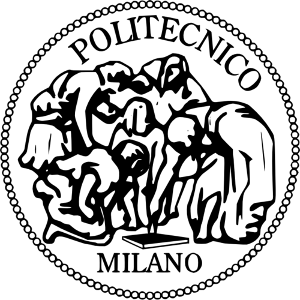
\includegraphics[width=5cm]{img/polimi_logo.png} % also works with logo.pdf
		\vfill
		{\bfseries\Large
			Travlendar+\\
			Requirement Analysis and Specification Document
			Version 0.1\\
			\vskip4cm
			Leonardo Bisica\\
			Alessandro Castellani\\
			Michele Cataldo\\
		}
		\vfill
		\vfill
	\end{titlepage}

	%%% table of contents %%%
	\tableofcontents
	
	\newpage
%%% 1 - INTRODUCTION %%%
	\section{Introduction}
		\subsection{Purpose}
		
		This document is the \textit{Requirement Analysis and Specification Document} (from now on RASD) for the information system \textit{Travelandar+}.
		This application aims to help users in their everyday life by organizing their appointments and optimizing their travel means.
		No previous versions of this application have been developed. 
		We’ll start by describing Stakeholders’ aims (Goals), from which we obtain, subsequently, functional and nonfunctional requirements (\textit{Requirements} Section) useful to describe the system.
		In addition we will need two other sections to have a complete overview of the model: \textit{Constraints} Section is going to describe constraints about the system, while \textit{Domain Properties} Section is going to underline the limits forced by the world on our software.
		We'll analyze this first chapter to subsequently delve into scenarios and use cases for the application.
		
		%TODO	
		\subsubsection{Goals}
			\begin{enumerate}
	\item
		[G1] System allows guest user to register with an username ad and a password; to complete the procedure user should confirm by 

	\item
		[G2] System Login

	\item 
		[G3] Registered User can create meetings 
	\item 
		[G4] Registered User can edit meetings
	\item 
		[G5] The application can automatically compute a personalized selection of travel times between appointments to choose from
	\item
		[G6] User can choose a preferred solution among the best ones
	\item
		[G7] The application warns the user if locations are unreachable in the allotted time
	\item
		[G8] Allow users to put constraints on different travel means and limit carbon footprints
	\item
		[G9] The application features additional user’s privileged time spans
	\item
		[G10] The application allows to arrange the trips : tickets for public services
	\item	
		[G11] The application allows the nearest shared vehicle to be found
	\item
		[G12] The application can obtain the position of the device and consequently of its user
		
\end{enumerate}	


		
		\subsection{Scope}
		The aim of this project is to develop \textit{Travlendar+}, a calendar-based mobile application. 
		The main functionality of the system is helping people in scheduling their appointments by taking into account useful, external information regarding traffic, public transportation, weather, and the like. 
		Appointments could be scheduled through the entire region of Lombardy (Italy), and the main Italian cities connected via railway system. There could be several types of work meetings and personal appointments.
		Furthermore the system can help the user by allowing the purchase of public transportation tickets via the mobile application itself, or by reserving a car or a bike of a sharing system (whenever this is possible). In case of bad weather the system should find alternative moving solutions in order to replace walking paths, same goes with strikes and other relevant kinds of information. 
		Naturally, the system will also allow the registration of new users; as for the registration, the system requests both personal and payment information. After the registration succeeds, the user could immediately start scheduling his meetings.
		
		\subsection{Glossary}
			\begin{description}
				\item[User] 
				\begin{itemize}
					\item First name;
					\item Last name; 
					\item Email;
					\item Username;
					\item Password;
					\item Payment information; this in particular includes:
						\begin{itemize}
							\item Credit card owner;
							\item Credit card number;
							\item Credit card expiration date;
							\item CVV number.
						\end{itemize}
				\end{itemize}
				
				\item[Guest] We name 'guests' all the people who are using the interface of the system without being registered or logged in. Guests can't access any functionality of \textit{Travlendar+} except for the registration process and the log in. 
				\item[Operative Zone] We name Operative Zone the area within we can place the location of an event. For the time being the Operative Zone coincide with all the cities and places within italian peninsula that can be reached by simply consulting the Google APIs. Naturally, such an area may be expanded in the future.
				\item[Influence Zone] We name Influence Zone the area within whose borders the mobile application can not only give travel time by car and on foot (the minimum standard given to us by Google APIs) but also where Travlendar+ can rely at least on a single car and bike sharing service. For starting, the Influence Zone will coincide with the city of Milan.
				\item
				\item[Registered User] A registered User is a former guest who inserted his/her own credentials in the system. After previous login, a Registered User can then create events, work on the timetable and ultimately is the end-user of Travlendar+.
				\item[Timetable]
				\item[Vehicle Sharing services/systems and a Shared Vehicle] By vehicle sharing we do not inted referring to a generic 'car-pooling' service. The usage of a shared vehicle may be either one of two types, car or bike sharing. A vehicle within the system operates only within the boundaries and parking zones imposed by its service; it can be picked up by any user registered to its corresponding system, used for the required amount of time (even though a maximum time is always fixed) and then parked in an allowed zone, ready to be picked by up again by another user. Eahc sharing system possesses an individual API			
				\item[Mobile Application] By mobile application we refer to a program conceived for Android and iOS operative systems, based on touch interfaces and able to run on portable devices. The logic of the mobile application is the system.
				\item[Appointment] An appointment is an event well delimited both in time and space, requiring the presence and the direct investment, in our case, of the user who creates it. Appointments fall in two categories : work appointments (that are often referred also as meetings) and personal appointments (the broader set encapsulating all other kinds of appointments, mainly regarding personal and family life)
				\item[Warning] A warning is a notification given by Travlendar+ mobile application to the operating System it is hosted by. It behaves as a standard system notification.
				\item[Travel Logic] By travel logic we refer to the logic that processes the distances and the transportation time within our operative and influcence zones. In the case at hand, in this first implementation, we're going to adopt as Travel Logic the Google Maps APIs.
\end{description}

		
		\subsection{Revision History}
			No revision where done since first edition of this document.
			
		\subsection{Reference Document}
			\begin{itemize}
				\item[-] \textsf{Specification Document : Mandatory Project Assignments.pdf}
				\item[-] \textsf{IEEE International Standard ISO/IEC/IEEE 29148 2011-12-01}
			\end{itemize}
		
		\subsection{Document Structure}	
			This document is composed by 5 chapter:
\begin{description}
	\item[Introduction:] this section gives a brief explanation of the system to be. It helps the reader with regards to the terminology and glossary and it gives him information about the documents that were used as references. 
	
	\item[Overall Description:] in this section it will be provided a solid background for the requirements so that they will became easier to understand. The reader will see also some pieces of hardware and software used to create the model.
	
	\item[Specific Requirements:] this section provides more details on the aspects of the prevoius section. In particular is presented the difference between functional and nonfunctional requirementes in addition to their perferomance and the explanation of external interface requirements.
	
	\item[Formal Analysis  using Alloy:] in this chapter the reader will see Alloy model of the system and some outputs obtained by running the model.
	
	\item[Effort Spent:]  is a section dedicated to shows the number of hours of each authors spent for create the model. 
	
	\item[Reference:] addiotional material usuful for the completness of the RASD.
\end{description}

		


%%% 2 - OVERALL DESCRIPTION  %%%
	\newpage
	\section{Overall Description}
		\subsection{Product perspective}
			%cose a caso
			

			
		\subsection{Product functions}
		
		\hfill \\ \\ 
 We’ve already detailed the main goals of our mobile application in the first section of the current document; naturally, the aforementioned goals will be functions of Travlendar+.
Here though we submit an higher-level description of major functions to ease the understanding of our program to all interested parties.\\
		
	

		\begin{enumerate}

		\item
		[\textbf{2.2.1}] \textbf{Appointments Manager}
		
Our mobile application will let any registered user to view, create, modify and delete events, denoted by their type, their date and location. \\

		\item
		[\textbf{2.2.2}] \textbf{Travel Scheduling}

When a new appointment is inserted in the application timetable an immediate check is performed whether the location of the event can be reached in the allotted time on foot,by car, or by public transportation (referencing, in lack of additional information, to their default behaviour according to the date and time of the day).
Day by day, events and allotted times are periodically checked with live informations to ensure they’re feasible : a list of results is prompted to the user whenever he asks for it and he can express preferences and filter them.\\

		\item
		[\textbf{2.2.3}] \textbf{Payment Manager for Public Transportation}

Our mobile application will redirect registered users to payment portals through secure channels and it’ll be able to verify whether transaction succeeded or not by interfacing with external payment services.
Unfulfilled payment will result in an impossibility to go forward and will prompt the possibility to submit the data and restart the transaction.\\

		\item
		[\textbf{2.2.4}] \textbf{Car and Bike Sharing Integration}

The mobile app will be able to integrate external info about the availability and location of shared cars and bikes so that it will also allow their reservation.
Everything past this mark clearly outgrows the scope of our system and it shall be handled by the company that grants the service (same goes for eventual malfunctions or erratic behaviours). 
Travlendar+ will send send reservation requests to the selected company and will be able to record a rental acceptance notification (i.e., everything’s gone right in the provider’s rental system).\\


		\item
		[\textbf{2.2.5}] \textbf{Free Time spans}

Our system will grant the possibility to reserve free time spans : such breaks won’t be affected by scheduling and by the need to travel and registered users will be able to insert theme directly in the calendar.\\

		\end{enumerate}

			
		\subsection{User characteristics}
			%cose a caso 2	
			
		\subsection{Assumptions, dependencies and constraints}
			%si spiega da sola


%%% 3 - SPECIFIC REQUIREMENTS %%%
	\newpage
	\section{Specific Requirements}
		%%% A %%%
\subsection{External Interface Requirements}
				\begin{description}
					\item[User Interfaces]
					\item[Hardware Interfaces]
					\item[Software Interfaces]
					\item[Communication Interfaces]
				\end{description}

%%% B %%%						
\subsection{Functional Requirements}
	
\subsection{Functional Requirements}

We now adopt a goal-based approach to determine the requirements associated with each one of the goals we have elaborated in Chapter 1.\\
We'll start numbering and exploring the goals we submitted.

\begin{itemize}

            \item \textit{[G1]} System allows guest user to register with an username ad and a password; to complete the procedure user should confirm by 
               
                  \begin{itemize}
                        \item [R.1.1] System should let registering user choose an username and password
                        \item [R.1.2] Every username corresponds to a single user
                        \item [R.1.3] Duplicate usernames aren’t allowed
                        \item [R.1.4] Registering user can't be already registered
                        \item [R.1.5] An unregistered user is locked out the application and can only see registration page
                        \item [R.1.6] User has to confirm by mail his registration
                  \end{itemize}
             
\item \textit{[G2]} System Login

                  \begin{itemize}
                        \item [R.2.1] User must be already registered to perform correct login
                        \item [R.2.2] User must remember username and password
                        \item [R.2.3] Only a correct combination of username and password will grant access
                        \item [R.2.4] Application will implement a password retrieval mechanism
                  \end{itemize}
                  
\item \textit{[G3]} Registered User can create appointments 

 \begin{itemize}
                        \item [R.3.1] User has to be registered and logged in the system in order to create an
appointment
                        \item [R.3.2] Appointments can be divided into work appointments (or meetings) and personal appointments
                        \item [R.3.3] Appointments require a location and a starting time and an end time
                        \item [R.3.4] Appointments location must be within the boundaries of the operative zone
                        \item [R.3.5] The chosen location can be within the boundaries of the influence zone
                        \item [R.3.5] There cannot be appointments with the same name, location and time
                        \item [R.3.6] Based on already existing appointments, system checks suitability of created new entries
                        \item [R.3.7] Appointment start time can't precede the actual system time at the moment of inserting it                        
                  \end{itemize}
                  
\item \textit{[G4]} Registered Users can edit meetings

                  \begin{itemize}
                       \item  [R.4.1] A modified meeting must respect all the constraint imposed during the creation of a new meeting, as in [G3]
                       \item [R.4.2] A meeting can be modified up until its end time
                       \item [R.4.3] If the location of the meeting is modified it gets 
                       \item [R.4.4] If the location of the meeting is modified system behaves as if such an event was inserted for the first time, calculating all possibile conflicts with pre-existing events
                       \item [R.5.5] No limit actually exists on the amount of times an event can be modified
                       \item [R.5.6] 
                     


                  \end{itemize}

\item \textit{[G5]} The application can automatically compute a personalized selection of travel times between appointments to choose from

                  \begin{itemize}
                        \item [R.5.1] System verifies the travel mean is feasible for the submitted appointments
                        \item [R.5.2] According to the type of appointment, the system submits the data to corresponding external services
                        \item [R.5.3] Based on meeting type and time of day system ranks all the solutions
                        \item [R.5.4] Time is calculated by imposing a start position submitted by the user as specificied in [G12]
                  \end{itemize}
                  
\item \textit{[G6]} User can choose a preferred solution among the best ones 

                   \begin{itemize}
                        \item [R.6.1] User must be able to choose between ranked solutions
                        \item [R.6.2] The application arranges a navigable view of feasible solutions
                        \item [R.6.3] 
                  \end{itemize}
                  
\item \textit{[G7]} The application warns the user if locations are unreachable in the allotted time 

\item \textit{[G8]} Allow users to put constraints on different travel means and limit carbon footprints

\item \textit{[G9]} The application features additional user’s privileged time spans 

\item \textit{[G10]} The application allows to arrange the trips : tickets for public services

\item \textit{[G11]} The application allows the nearest shared vehicle to be found and reserved

                   \begin{itemize}
                        \item [R.11.1] A shared vehicle belongs to a bike-sharing service or a car-sharing service
                        \item [R.12.2] All services linked to shared vehicles are automatically disabled if the location of a meeting out of the boundaries of the influence zone
                        \item [R.12.3] All sharing services have their own API and they must be referenced by our mobile application
                        \item [R.12.4] To find or reserve a vehicle it is required by our system the access to the external API of the required service
                        \item [R.12.5] To find or reserve a vehicle it's required that the user logins into the external corresponding service
                        \item [R.12.6] The external service can communicate with our mobile application. In case of reservation Travlendar+ checks if the mobile app corresponding to the desired services is installed on the system. All the following steps take place within such an environment, until control is returned to Travlendar+
                        \item [R.12.7] The location of all the vehicles are shown in the same view, merging data from different APIs
                        \item [R.12.8] The renting happens 
                        
                        
                    \end{itemize}

\item \textit{[G12]} The application can obtain the position of the device and consequently of its user
                   
                  \begin{itemize}
                        \item [R.12.1] User can manually insert a location
                        \item [R.12.2] The mobile device can track its current position through geo-localization
                        \item [R.12.3] Position of out the operative zone won't be accepted by the system
                   \end{itemize}


\item \textit{[G13]} EVENTUAL NAVIGATION


    

			
%%% C %%%
\subsection{Performance Requirements}
		
		
%%% D %%%	
\subsection{Design Constraints}
		\begin{description}
			\item[Standards compliance]
			\item[Hardware limitations]
			\item[Any other constraint]
		\end{description}
		
%%% E %%%		
\subsection{Software System Attributes}
	\begin{description}
		\item[Reliability]
		\item[Availability]
		\item[Security]
		\item[Maintainability]
		\item[Portability]
\end{description}


%%% 4 - SCENARIOS %%%
	\newpage
	\section{Scenarios}
		\subsection{Scenario "2"}

David is 17 years old and has recently joined the soccer team of his city. His coach has fixed that training sessions will be held every Monday, Wednesday and Friday at 18:00. Then David opens Travelandar+ and puts his commitments until the end of the season. The application suggests that the fastest way to go to the field training is the subway, so David decides to buy a season pass so that he can safely go to training sessions without having to ask his parents.\\
After buying season pass he registered it on the application.

% Latex non conta gli "a capo" che fai con "enter", ma solamente con il doppio backslash \\
% quindi sentiti libero di impagninarlo come meglio credi

\subsection{Scenario "3"}

Elizabeth loves dedicating the right amount of time to her appointments, from work to family to her hobbies. Recently though she’s having a hard time conciling all of her commitments. 
That’s why her friend Alex recommends her to use the Travelandar + application : Elizabeth follows his advice and downloads the application on her smartphone. 
It’s only half an hour and Elisabetta is very satisfied, especially because she could set up an "Optimal Lunch" function that allows her to devote the right amount of time to her lunch, denying the opportunity to add appointments around the 30 minutes dedicated to lunch.

\subsection {Scenario "4"}
John had an hard day, he’s just put the finishing touches on his project : he had to work even during this weekend, locked at home. Just when he’s done with his assignment he receives an invitation to go out and see a movie with Jane and the rest of his friends. 
He’s in a rush and he hasn’t previously registered such an appointment in his calendar; to make things worse, he doesn’t own a car, and public transportation is rather slow in the weekend. Because of this he rules out both car and the public transportation as travel means, and when he inserts location and time of the unexpected appointment only car sharing pops up as a viable and fast option. 
John obviously accepts and rents the car through Travlendar+. 


\subsection{Scenario "8"}

Tom is a bank employee working in Bologna. He decided to return at home in Milan next Friday to celebrate his father's birthday together with his family. Because of this he opens Travlendar+ on his smartphone and creates a "Dad's party" event for Friday night. Tom’s job does not allow him to leave Bologna before 18.00. Fortunately Travlendar+ also allows him to find travel solutions by cross-region trains as well as by car. In fact, it all comes down to Tom's choice. He proceeds to buy train tickets : to him Friday isn’t coming fast enough!


%%% 5 - ALLOY %%%
	\newpage
	\section{Alloy modeling}


%%% 6 - APPENDIX %%%
	\newpage	
	\section{Appendix}
		\listoffigures
		\listoftables
		
		\subsection{Used tools}
		For this assignment, we used the following tools:
		
		\begin{description}
			\item [Alloy] We used the alloy tool to write the code and check the models for the specification.
			\item [LaTeX] The group used LaTeX to structure the final document and to help with versioning.
			\item [Github] We leaned on Github for versioning and coordinating synchronized work.
			
		\end{description}
		
		\subsection{Hours of work}
			\begin{description}
				\item[Bisica, Leonardo] around xx hours of work;
				\item[Castellani, Alessandro] around xx hours of work;
				\item[Cataldo, Michele] around xx hours of work.
			\end{description}
			
\end{document}
